\documentclass[a4paper]{article}
\usepackage{student}
\usepackage{hyperref}
\usepackage{graphicx}
\usepackage{algorithm}
\usepackage{algorithmic}
\usepackage{breqn}
\usepackage{subcaption}
\usepackage{multirow}
\usepackage{psfrag}
\usepackage{url}
\usepackage{hyperref}
%\usepackage[colorlinks]{hyperref}
\usepackage{cleveref}
\usepackage{booktabs}
\usepackage{rotating}
\usepackage{colortbl}
\usepackage{paralist}
%\usepackage{geometry}
\usepackage{epstopdf}
\usepackage{nag}
\usepackage{microtype}
\usepackage{siunitx}
\usepackage{nicefrac}
% for random text
\usepackage{lipsum}
\usepackage[english]{babel}
\usepackage[pangram]{blindtext}
% for tikz figures
\usepackage{listings}
\usepackage{tikz}
\usetikzlibrary{fit,positioning,arrows.meta,shapes,arrows}
% Metadata
\date{\today}
\setmodule{SIT742: Modern Data Science}
\setterm{Trimester 2, 2024}

%-------------------------------%
% Other details
% TODO: Fill these
%-------------------------------%
\title{Assignment 2}
\setmembername{SIT742}  % Fill group member names
%\setmemberuid{u1234567, u7654321}  % Fill group member uids (same order)

%-------------------------------%
% Add / Delete commands and packages
% TODO: Add / Delete here as you need
%-------------------------------%
\usepackage{amsmath,amssymb,bm}

\newcommand{\KL}{\mathrm{KL}}
\newcommand{\R}{\mathbb{R}}
\newcommand{\E}{\mathbb{E}}
\newcommand{\T}{\top}

\newcommand{\expdist}[2]{%
        \normalfont{\textsc{Exp}}(#1, #2)%
    }
\newcommand{\expparam}{\bm \lambda}
\newcommand{\Expparam}{\bm \Lambda}
\newcommand{\natparam}{\bm \eta}
\newcommand{\Natparam}{\bm H}
\newcommand{\sufstat}{\bm u}

% Main document
\begin{document}
    % Add header
    \header{}



    \begin{center}
        \fbox{\fbox{\parbox{5.5in}{\centering
\begin{description}
    \item [Extension Request] 
    Students with difficulty in meeting the deadline 
    because of various reasons,
    must apply for an assignment extension 
    no later than 5:30pm on 20/09/2024 (Friday).
    Apply via `\texttt{CloudDeakin}', 
    the menu item `\texttt{Extension Request}' 
    under the `\texttt{Assessment}' drop-down menu. 
    \item[\href{https://www.deakin.edu.au/students/studying/academic-integrity}{Academic Integrity}] 
    All assignment will be checked for plagiarism, 
    and any academic misconduct will be reported to 
    unit chair and university.

    \item[Generative AI] Deakin's Policy and advices on responsible usage of Generative AI in your studies: \url{https://www.deakin.edu.au/students/study-support/study-resources/artificial-intelligence}
\end{description} 
}}}
 
      \end{center}

      \section*{Instructions}


      \subsection*{Assignment Questions}\label{sec:question}
      
      There are total \textbf{2} parts in the assessment task 2:
      \begin{description}
      \item[Part $1$] 
      The first part will focus on the data manipulation and pyspark skills
      which includes the \texttt{Data Acquisition}, the \texttt{Data Wrangling}, the \texttt{EDA} and \texttt{Spark},
      the \texttt{modules and library} from \href{https://github.com/tulip-lab/sit742/tree/develop/Jupyter/}{\textbf{M03, M04}}.
          
      \item[Part $2$] 
      The second part focus on more advanced data science skills with particular scenario. 
      This part will require the knowledge covered in \href{https://github.com/tulip-lab/sit742/tree/develop/Jupyter/M05-DataAnalytics}{\textbf{M05}}.
      \end{description}
      

    
\subsection*{What to Submit?}\label{sec:submit}

There is \textcolor{red}{no optional part for assignment 2}.
You (your group) are required to 
submit the following completed files to 
the corresponding \emph{Assignment} (Dropbox) in \emph{CloudDeakin}:
\begin{description} 
\item[\texttt{SIT742Task2.ipynb}] 
The completed notebook with \texttt{all the run-able code} for all requirements (part 1 and part2).

In general, 
you (your group) need to complete, 
\textcolor{red}{\textbf{save}} the results of running, 
download/export the notebook as a local file,
and submit your \textbf{notebook} 
from Python platform such as \texttt{Google Colab}. 
You need to clearly list the answer for each question,
and the expected format from your notebook will 
be like in~\Cref{fig:format} (\textbf{One notebook} for each group).

\begin{figure}[H]
    \centering
    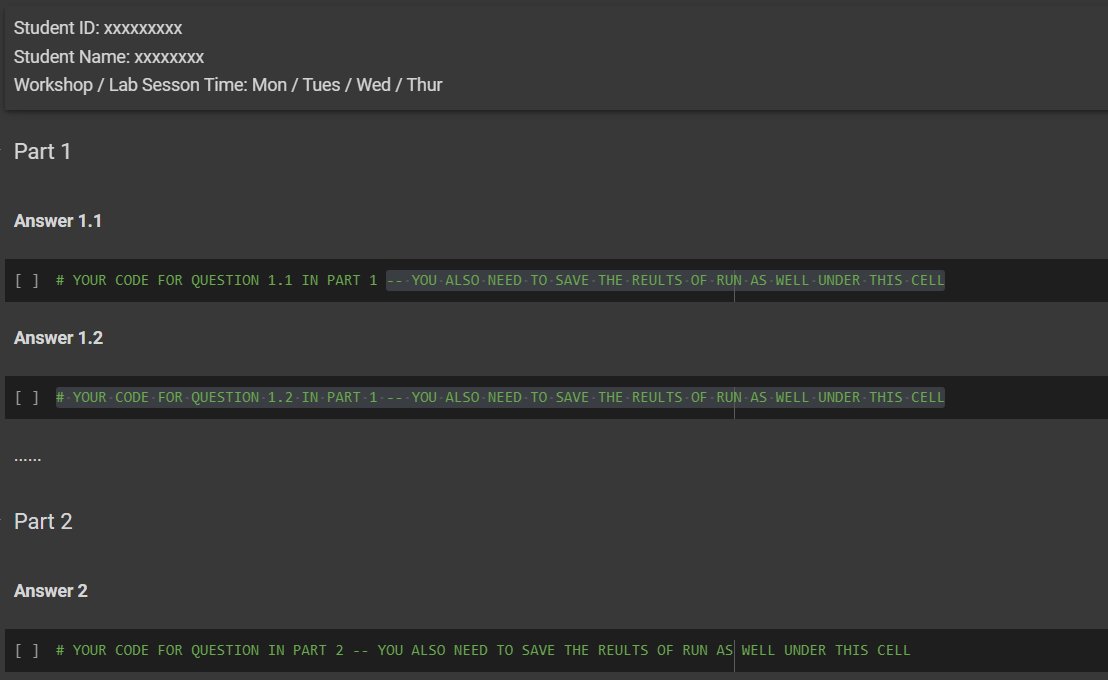
\includegraphics[width=0.99\columnwidth]{figure/assigment1.png}
    \caption{Notebook Format}
    \label{fig:format}
\end{figure}
    

\item[\texttt{SIT742Task2report.pdf}] 
You (group) are also required to write a report with 
your answer (code) and running results from \texttt{SIT742Task2.ipynb} for all the questions (\texttt{Part 1} and \texttt{Part 2}).
You could make screenshot on your answer (code) and running results from \texttt{SIT742Task2.ipynb} and paste into the report.
Please try to include the code comments, and results including plot images as well in the report,
and make sure
the code format such as Indentation keeps same as the ipynb notebook. 

In this report (\textbf{one for each group}), 
you will also need to provide a clear explanation on your logic for solving each question (you could write explanation below your solution and results in the report).
In the explanation, you will need to cover below parts:
1). why you decide to choose your solution;
2). are there any other solutions that could solve the question;
3). whether your solution is the optimal or not? why?
The length of the explanation part for each question is limited below $100$ words.

In the end of your report, 
you (group) also need to discuss below three points:
\begin{itemize}
    \item How you and your team member collaborate on this assignment? 
    \item What you have learned with your team member from the second assignment.
    \item What is the contribution of each the team member for finishing the second assignment.
\end{itemize}

\item[\texttt{SIT742Task2video.avi}] 
A video demonstration between $10$ and $15$ minutes,
and the file format can be any common video format,
such as `\texttt{MKV}', `\texttt{WMV}', `\texttt{MOV}' etc. 

For your group,
one important submission is a \textbf{short video} 
in which each of \emph{You} (group members) orally present the solutions 
that you provide in the notebook 
and illustrate the running of code with the used logic.
In the video, 
your group need to work together to discuss below three points:
\begin{itemize}
    \item Which question(s) you have worked on and how did you collaborate with other team members.
    \item What is the logic behind the your solution on the question(s)? and is there any alternative optimized ways to resolve the question?
    \item What is your understanding of \texttt{Code collaboration}? How do you collaborate with your group in coding? What are the common tools/platform to support the \texttt{Code collaboration}?
\end{itemize}
\end{description}


     
    \part{Data Acquisition and Manipulation}\label{sec:part1}

    There are \textbf{10} questions in this part, totalling \textbf{60} marks. 
    Each of question is worth \textbf{5} marks. Additionally, the quality of your explanation in both the report and video will collectively be worth \textbf{10} marks.
    
    
    You are recommended to use \texttt{Google Colab} to 
    finish all the coding in the \textit{code block cell},
    and \textcolor{red}{provide sufficient coding comments},
    and also \textcolor{red}{save the result of running as well}. 

    The (\texttt{transactionrecord.zip}) data used for this part could be found in 
    \href{https://github.com/tulip-lab/sit742/blob/develop/Assessment/2024/data/transactionrecord.gz}{\textbf{here}}.
    You will need to use \texttt{spark} to read the unzipped (csv) data for starting.
    You could find the code on reading csv data with Spark from \href{https://github.com/tulip-lab/sit742/blob/develop/Jupyter/M04-DataManipulation/M04G-SparkSQL.ipynb}{M04G}.
    
    \begin{answer}[Question 1.1] 
        Using PySpark to do some of the data wrangling process, so that:
        \begin{description}
            \item[1.1.1] For the \texttt{'NA'} in \texttt{CustomerNo} columns, change it to \texttt{'-1'}.
            \item[1.1.2] Process the text in \texttt{productName} column, only alphabet characters left, and save the processed result to a new column \texttt{productName_process} and show the first 5 rows.

        \end{description}
    
    \end{answer}
    
    \begin{answer}[Question 1.2]
    Find out the revenue on each transaction date. In order to achieve the above, some wrangling work is required to be done:
     \begin{description}
            \item[1.2.1] Using \texttt{pyspark} to calculate the \texttt{revenue} (\texttt{price} * \texttt{Quantity}) and save as float format in pyspark dataframe to show the top 5 rows.
            \item[1.2.2] Transform the pyspark dataframe to \texttt{pandas} dataframe (named as \texttt{df}) and create the column \texttt{transaction_date} with date format according to {Date}. Print your \texttt{df} pandas dataframe with top 5 rows after creating the column \texttt{transaction_date}.
            \item[1.2.3] Plot the sum of \texttt{revenue} on  \texttt{transaction_date} in a line plot and find out any immediate pattern / insight?
    \end{description}
    \end{answer}
    
    \begin{answer}[Question 1.3]
    Let's continue to analyse on the \texttt{transaction_date} vs \texttt{revenue}. 
    \begin{description}
        \item[1.3.1] Determine which \texttt{workday} (day of the week),
  generates the most sales (plotting the results in a line chart with workday on averaged revenues).
        \item[1.3.2] Identify the name of product (column \texttt{productName_process}) that contributes the highest revenue on `\texttt{that workday}' (you need to find out from 1.3.1) and the name of product (column \texttt{productName_process}) that has the highest sales volume (sum of the \texttt{Quantity}), no need to remove negative quantity transactions.) on `\texttt{that workday}' (you need to find out from 1.3.1).
        \item[1.3.3] Please provide two plots showing the top 5 products that contribute the highest revenues in general and top 5 products that have the highest sales volumes in general.
    \end{description}
    
    \end{answer}
    
    \begin{answer}[Question 1.4]
    Which country generates the highest revenue? Additionally, identify the month in that country that has the highest revenue.
    \end{answer}
    
    \begin{answer}[Question 1.5]
    Let's do some analysis on the \texttt{CustomerNo} and their transactions.
    Determine the shopping frequency of customers to identify who shops most frequently (find out the highest distinct count of \texttt{transactionNo} on customer level, be careful with those transactions that is not for shopping -- \texttt{filter those transaction quantity <= 0}). Also, find out what products (column \texttt{productName_process}) `\texttt{this customer}' typically buys based on the \texttt{Quantity} of products purchased. 
    
    \end{answer}
    
    
    \begin{answer}[Question 1.6]
    As the data scientist, you would like to build a basket-level analysis on the product customer buying (filter the `\texttt{df}' dataframe \texttt{with df['Quantity']>0}).
    In this task, you need to:
    \begin{description}
        \item[1.6.1] Group by the \texttt{transactionNo} and aggregate the category of product (column \texttt{product_category}) into list on \texttt{transactionNo} level.
        Similarly, group and aggregate name of product (column \texttt{productName_process}) into list on \texttt{transactionNo} level.
        \item[1.6.2] Removing duplicates on adjacent elements in the list from \texttt{product_category} you obtained from 1.6.1, such as \texttt{[product category 1, product category 1, product category 2, ...]} will be processed as \texttt{[product category 1, product category 2,....]}. After this processing, there will be no duplicates on on adjacent elements in the list. Please save your processed dataframe as `\texttt{df_1}' and print the top 10 rows.
    \end{description}
    \end{answer}
    
    
    \begin{answer}[Question 1.7]
    Continue work on the results of question 1.6, now for each of the transaction, you will have a list of product categories. To further conduct the analysis, you need to finish below by using dataframe `\texttt{df_1}':

    \begin{description}
        \item[1.7.1] Create new column \texttt{prod_len} to find out the length of the list from \texttt{product_category} on each transaction. Print the first five rows of dataframe `\texttt{df_1}'.
        \item[1.7.2] Transform the list in \texttt{product_category} from \texttt{[productcategory1, productcategory2...]}
        to `\texttt{start > productcategory1 > productcategory2 > ... > conversion}'
        with new column \texttt{path}. You need to add `\texttt{start}' as the first element, and `\texttt{conversion}' as the last. Also you need to use `\texttt{ > }' to connect each of the transition on products (there is a space between the elements and the transition symbol \texttt{>}).
        The final format after the transition is given in example as below \cref{fig:1.7q}.
        Define the function \texttt{data_processing} to achieve above with three arguments: \texttt{df} which is the dataframe name, \texttt{maxlength} with default value of 3 for filtering the dataframe with \texttt{prod_len" <=maxlength} and \texttt{minlength} with default value of 1 for filtering the dataframe with \texttt{prod_len >=minlength}.
        The function \texttt{data_processing} will return the new dataframe `\texttt{df_2}'. Run your defined function with dataframe `\texttt{df_1}', \texttt{maxlength = 5} and \texttt{minlength = 2}, print the dataframe `\texttt{df_2}' with top 10 rows.
    \end{description}
    \begin{figure}[H]
        \centering
        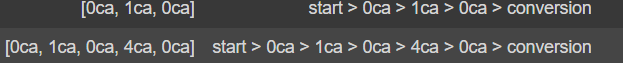
\includegraphics[width=0.85\columnwidth]{figure/1.7_figure.png}
        \caption{Example of the transformation on 1.7.2, left column is before the transformation, right column is after the transformation. After transformation, it is not list anymore}
        \label{fig:1.7q}
    \end{figure}

    Hint: you might consider to use \texttt{str.replace()} syntax from default python 3.
    \end{answer}
    
    
    \begin{answer}[Question 1.8]
     Continue to work on the results of question 1.7, the dataframe `\texttt{df_2}', we would like to build the \texttt{transition matrix} together, but before we actually conduct the programming, we will need to finish few questions for exploration:

     \begin{description}
         \item[1.8.1] Check on your transaction level basket with results from question 1.7, could you please find out respectively how many transactions ended with pattern `\texttt{... > 0ca > conversion}' / `\texttt{... > 1ca > conversion}' / `\texttt{... > 2ca > conversion}' / `\texttt{... > 3ca > conversion}' / `\texttt{... > 4ca > conversion}' (1 result for each pattern, total 5 results are expected).

         \item[1.8.2] Check on your transaction level basket with results from question 1.7, could you please find out respectively how many times the transactions contains `\texttt{0ca > 0ca}' / `\texttt{0ca > 1ca}' / `\texttt{0ca > 2ca}' / `\texttt{0ca > 3ca}' / `\texttt{0ca > 4ca}' / `\texttt{0ca > conversion}' in the whole data (1 result for each pattern, total 6 results are expected and each transaction could contain those patterns multiple times, such as `\texttt{start > 0ca > 1ca > 0ca > 1ca > conversion}' will count `\texttt{two}' times with pattern `\texttt{0ca > 1ca}', if there is not any, then return 0, you need to sum the counts from each transaction to return the final value).

         \item[1.8.3] Check on your transaction level basket with results from task question 1.7, could you please find out how many times the transactions contains `\texttt{...> 0ca > ...}' in the whole data (1 result is expected and each transaction could contain the pattern multiple times, such as `\texttt{start > 0ca > 1ca > 0ca > 1ca > conversion}' will count `\texttt{two}' times, you need to sum the counts from each transaction to return the final value).

         \item[1.8.4] Use the 6 results from 1.8.2 to divide the result from 1.8.3 and then sum all of them and return the value.
     \end{description}

     Hint: you might consider to use \texttt{endswith} and \texttt{count} functions from default python 3.
     
    \end{answer}


    \begin{answer}[Question 1.9]
    Let's now look at the question 1.6 again, you have the list of product and list of product category for each transaction. We will use the \texttt{transactionNo} and \texttt{productName_process} to conduct the Association rule learning.

    \begin{description}
        \item[1.9.1] Work on the dataframe \texttt{df} from question 1.2 (filter out the transaction with negative quantity value and also only keep those top 100 products by ranking the sum of quantity) and build the transaction level product dataframe (each row represents \texttt{transactionNo} and \texttt{productName_process} become the columns, the value in the column is the \texttt{Quantity}). \\
        Hint: you might consider to use \texttt{pivot} function in pandas.
        \item[1.9.2] Run the apriori algorithm to identify items with minimum support of 1.5\% (only looking at baskets with 4 or more items). \\
        Hint: you might consider to use \texttt{mlxtend.frequent_patterns} to run apriori rules.

        \item[1.9.3] Run the apriori algorithm to find the items with \texttt{support >= 1.0\%} and \texttt{lift > 10}. 

        \item[1.9.4] Please explore three more examples with different support / confidence / lift measurements (you could leverage your rule mining with one of the three measurements or all of them) to find out any of the interesting patterns from the Association rule learning. Save your code and results in a clean and tidy format and writing down your insights.
    \end{description}
    \end{answer}

    \begin{answer}[Question 1.10]
     After we finished the Association rule learning, it is a time for us to consider to do customer analysis based on their shopping behaviours.

     \begin{description}
         \item[1.10.1]  Work on the dataframe \texttt{df} from question 1.2 and build the customer product dataframe (each row represents single \texttt{customerNo} and \texttt{productName_process} become as the columns, the value in the columns is the aggregated \texttt{Quantity} value from all transactions and the result is a N by M matrix where N is the number of distinct \texttt{customerNo} and M is the number of distinct \texttt{productName_process}. Please filter out the transaction with negative quantity value and also only keep those top 100 product by ranking the sum of quantity).
         
         \item[1.10.2] Use the customer-product dataframe, let's calculate the Pairwise Euclidean distance on customer level (you will need to use the product Quantity information on each customer to calculate the Euclidean distance for all other customers and the result is a N by N matrix where N is the number of distinct \texttt{customerNo}). 

         \item[1.10.3]  Use the customer Pairwise Euclidean distance to find out the top 3 most similar customer to \texttt{CustomerNo == 13069} and \texttt{CustomerNo == 17490}. 

         \item[1.10.4]  For the customer \texttt{CustomerNo == 13069}, you could see there are some products that this customer has never shopped before, could you please give some suggestions on how to recommend these product to this customer? please write down your suggestions and provide a coding logic (steps on how to achieve, not actual code).
     \end{description}
    \end{answer}
    
    \part{Sales Prediction}\label{sec:part2}

    There are \textbf{3} questions in this part,
    totaling \textbf{40} marks.
    Each question is worth \textbf{10} marks. 
    Additionally,
    the quality of your explanation in both the report and video will collectively be worth \textbf{10} marks. 
    
    You are required to use \texttt{Google Colab} to 
    finish all the coding in the \textit{code block cell},
    and \textcolor{red}{provide sufficient coding comments},
    and also \textcolor{red}{save the result of running as well}. 

    In this part, we will focus only on two columns \texttt{revenue} with \texttt{transaction_date} to form the revenue time series based on \texttt{transaction_date}.
    We will use the dataframe \texttt{df} from question 1.2 (without any filtering on transactions) to finish below sub-tasks:

    
    \begin{answer}[Question 2.1]
    You are required to explore the revenue time series.
    There are some days not available in the revenue time series such as \texttt{2019-01-01}.
    Please add those days into the revenue time series with default revenue value with 
    the mean value of the revenue in the whole data (without any filtering on transactions).
    After that, decompose the revenue time series with addictive mode and analyses on the results to find if there is any seasonality pattern (you could leverage the \texttt{M05A} material from lab session with default setting in \texttt{seasonal_decompose} function).
    
    \end{answer}

    \begin{answer}[Question 2.2]
    We will try to use time series model \texttt{ARIMA} for forecasting the future. you need to find the best model with different parameters on \texttt{ARIMA} model. The parameter range for p,d,q are all from \texttt{[0, 1, 2]}. In total, you need to find out the best model with lowest \texttt{Mean Absolute Error} from 27 choices based on the time from ”Jan-01-2019” to ”Nov-01-2019” (you might need to split the time series to train and test with grid search according to the \texttt{M05B} material).
    \end{answer}

    \begin{answer}[Question 2.3]
    There are many deep learning time series forecasting methods, could you please explore those methods and write down the necessary data wrangling and modeling steps (steps on how to achieve, not actual code). Also please give the reference of the deep learning time series forecasting models you are using.
    \end{answer}
    
    
    
\end{document}
